\documentclass[10pt]{article}
\usepackage[margin=0.5in]{geometry}
\usepackage{color}
\usepackage{graphicx}
\usepackage{epstopdf}
\epstopdfsetup{update}
\usepackage{amsmath}
\usepackage{amssymb}
\usepackage[colorlinks]{hyperref}
\usepackage{geometry}
\usepackage[square]{natbib} 

\newcommand{\bea}{\begin{eqnarray}}
\newcommand{\eea}{\end{eqnarray}}
\newcommand{\bF}{\mathbf{F}}
\newcommand{\ba}{\mathbf{a}}
\newcommand{\bA}{\mathbf{A}}
\newcommand{\bu}{\mathbf{u}}
\newcommand{\bg}{\mathbf{g}}
\newcommand{\bB}{\mathbf{B}}
\newcommand{\bd}{\mathbf{d}}
\newcommand{\be}{\mathbf{e}}
\newcommand{\bm}{\mathbf{m}}
\newcommand{\bM}{\mathbf{M}}
\newcommand{\bv}{\mathbf{v}}
\newcommand{\bV}{\mathbf{V}}
\newcommand{\bp}{\mathbf{p}}
\newcommand{\bP}{\mathbf{P}}
\newcommand{\br}{\mathbf{r}}
\newcommand{\bx}{\mathbf{x}}
\newcommand{\bR}{\mathbf{R}}
\newcommand{\bN}{\mathbf{N}}
\newcommand{\bell}{\boldsymbol{\ell}}
\newcommand{\bL}{\mathbf{L}}
\newcommand{\btau}{\boldsymbol{\tau}}
\newcommand{\bT}{\mathbf{T}}
\newcommand{\bi}{\mathbf{i}}
\newcommand{\bj}{\mathbf{j}}
\newcommand{\bk}{\mathbf{k}}
\newcommand{\bn}{\mathbf{n}}
\newcommand{\bomega}{\boldsymbol{\omega}}
\newcommand{\md}{\mathrm{d}}
\newcommand{\ie}{\textit{i.e.{ }}}
\newcommand{\etc}{\textit{etc.{ }}}
\newcommand{\ddt}{\frac{\md}{\md t}}
\newcommand{\ddtt}{\frac{\md^2}{\md t^2}}
\newcommand{\ppt}{\frac{\partial}{\partial t}}
\newcommand{\pptt}{\frac{\partial^2}{\partial t^2}}
\newcommand{\me}{\mathrm{e}}


%===============================================
\begin{document}
\title{Two-points umklapp model}
%\author{Da Wang}%\thanks{dawang@nju.edu.cn} \\ \\National Laboratory of Solid State Microstructures $\&$ School of Physics, \\ Nanjing University, Nanjing, 210093, China}
\date{}
\maketitle

%\begin{abstract}
We are seeking a diagrammatic treatment of the two-points umklapp model. It seems we are doing a trick
\bea \sum_k\int\mathcal{D}\phi \ne \int\mathcal{D}\phi\sum_k \eea
In fact, the strategy is somewhat in parallel with Hertz (1976). 
%\end{abstract}

%\tableofcontents
%=================================================
The model is defined as
\bea H=gR_\uparrow^\dag R_\downarrow^\dag L_\downarrow L_\uparrow + h.c. \eea

\section{HS field representation}
The partition function is
\bea Z&=&\int{ \mathcal{D}R\mathcal{D}L \me^{\int{ \bar{R}_\sigma (-\partial\tau)R_\sigma + \bar{L}_\sigma (-\partial\tau)L_\sigma -g(\bar{R}_\uparrow \bar{R}_\downarrow L_\downarrow L_\uparrow + h.c.)} }} \\
&=&\int{ \mathcal{D}R\mathcal{D}L \me^{\int {\bar{R}_\sigma (-\partial\tau)R_\sigma + \bar{L}_\sigma (-\partial\tau)L_\sigma +g(\bar{R}_\uparrow \bar{R}_\downarrow-\bar{L}_\uparrow \bar{L}_\downarrow)(R_\downarrow R_\uparrow-L_\downarrow L_\uparrow) - g\bar{R}_\uparrow \bar{R}_\downarrow R_\downarrow R_\uparrow -g \bar{L}_\uparrow \bar{L}_\downarrow L_\downarrow L_\uparrow}}}  \\
&=&\int{ \mathcal{D}R\mathcal{D}L\mathcal{D}\phi \me^{ \int{  \bar{R}_\sigma (-\partial\tau)R_\sigma + \bar{L}_\sigma (-\partial\tau)L_\sigma +[\phi (\bar{R}_\uparrow \bar{R}_\downarrow-\bar{L}_\uparrow \bar{L}_\downarrow) + h.c.]-\frac1g\phi^*\phi  - g\bar{R}_\uparrow \bar{R}_\downarrow R_\downarrow R_\uparrow -g \bar{L}_\uparrow \bar{L}_\downarrow L_\downarrow L_\uparrow }}} \\
&=&\int \mathcal{D}R\mathcal{D}L\mathcal{D}\phi \sum_k \frac{(-g)^k}{k!} \int \md^k\tau \mathcal{T}_\tau (\bar{R}_\uparrow \bar{R}_\downarrow R_\downarrow R_\uparrow +\bar{L}_\uparrow \bar{L}_\downarrow L_\downarrow L_\uparrow)^k \nonumber\\ 
&&  \me^{ \int{  \bar{R}_\sigma (-\partial\tau)R_\sigma + \bar{L}_\sigma (-\partial\tau)L_\sigma +[\phi (\bar{R}_\uparrow \bar{R}_\downarrow-\bar{L}_\uparrow \bar{L}_\downarrow) + h.c.]-\frac1g\phi^*\phi  }} \\
&\rightarrow&\int \mathcal{D}\phi\sum_k\frac{(-g)^k}{k!}\int \md^k\tau\mathcal{T}_\tau(\partial_{\eta_\uparrow}\partial_{\eta_\downarrow}\partial_{\bar{\eta}_\downarrow}\partial_{\bar{\eta}_\uparrow}+\partial_{\xi_\uparrow}\partial_{\xi_\downarrow}\partial_{\bar{\xi}_\downarrow}\partial_{\bar{\xi}_\uparrow})^k \nonumber\\&& \me^{\mathrm{Tr}\log(\partial_\tau+\hat{\phi})+\mathrm{Tr}\log(\partial_\tau-\hat{\phi})+\bar{\eta}(\partial_\tau+\hat{\phi})^{-1}\eta+\bar{\xi}(\partial_\tau-\hat{\phi})^{-1}\xi-\frac1g\phi^*\phi} \\
&=& \int \mathcal{D}\phi \sum_k \frac{(-g)^k}{k!}\int \md^k\tau \mathcal{T}_\tau (\partial_{\eta_\uparrow}\partial_{\eta_\downarrow}\partial_{\bar{\eta}_\downarrow}\partial_{\bar{\eta}_\uparrow}+\partial_{\xi_\uparrow}\partial_{\xi_\downarrow}\partial_{\bar{\xi}_\downarrow}\partial_{\bar{\xi}_\uparrow})^k \me^{S[\phi,\eta,\xi]} \eea
where we have introduced the source $\eta$ and $\xi$ coupled to $R$ and $L$, respectively. 
The exact Green's function $G_R$ is given by
\bea \hat{G}_R&=&\frac{1}{Z}\int \mathcal{D}\phi \sum_k \frac{(-g)^k}{k!} \int\md^k\tau\mathcal{T}_\tau \partial_{\bar{\eta}} \partial_\eta (\partial_{\eta_\uparrow}\partial_{\eta_\downarrow}\partial_{\bar{\eta}_\downarrow}\partial_{\bar{\eta}_\uparrow}+\partial_{\xi_\uparrow}\partial_{\xi_\downarrow}\partial_{\bar{\xi}_\downarrow}\partial_{\bar{\xi}_\uparrow})^k \me^{S[\phi,\eta,\xi]} \\
&=&\frac{\int\mathcal{D}\phi \left[\sum {\rm connected}\right]_\phi\left[\sum {\rm closed}\right]_\phi \me^{S[\phi]} }{\int\mathcal{D}\phi \left[\sum {\rm closed}\right]_\phi \me^{S[\phi]}}
\eea
Clearly, if without $\phi$, the closed diagrams can be canceled. But when $\phi$ exists, we cannot do such a simplification unless $|\phi|$ is pinned at a fixed value like in $T=\infty$ and $T=0$ limits. The former is just the usual diagrammatic expansion while the latter is the mean field theory. 

Next, let us seek an (semi-)analytical treatment. Let's first try the approximation of $\phi(\tau)=\phi$, \ie time independent. Then, $\int \mathcal{D}\phi\rightarrow\int\md\phi$ and
\bea S(\phi)=2\log(1+\me^{-\beta|\phi|})+2\log(1+\me^{\beta|\phi|})-\frac{\beta|\phi|^2}{g} \eea  

A second approximation is to truncate $k$ with a upper bound $N_k$. When $N_k=0$, we have omitted all closed diagrams, \ie $\sum[{\rm closed}]=1$. Then, we have
\bea G_R=\left. \int\md \phi \frac{1}{2}\left(\frac{1}{i\omega_n-|\phi|}+\frac{1}{i\omega_n+|\phi|}\right) \me^{S(\phi)}  \middle/ \int\md  \phi \me^{S(\phi)}\right. \eea

Next, let's set $N_k=1$. However, the result becomes worse. The reason is the amplitude fluctuations can not be neglected in the middle temperature regime.  
\begin{figure}[h]
    \begin{center}
    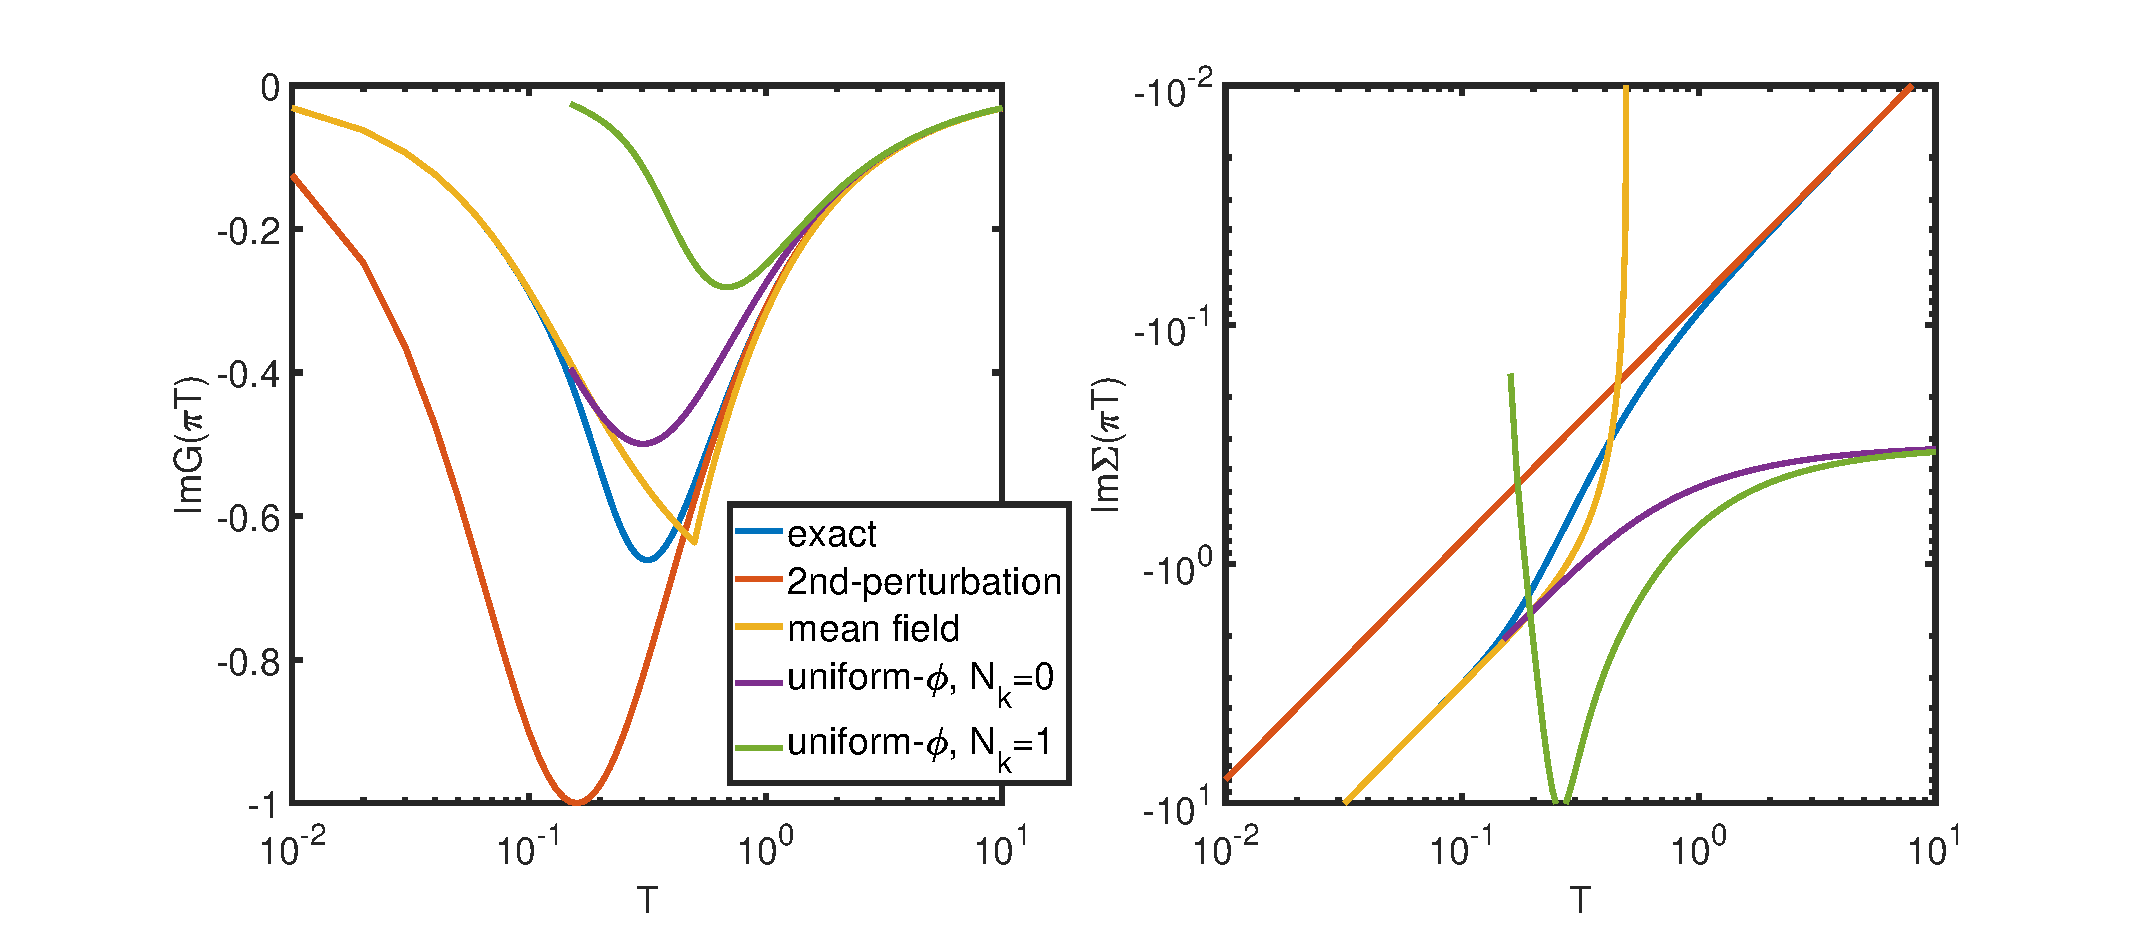
\includegraphics[width=0.8\textwidth]{result.eps}
    \caption{Approximation of time-independent $\phi$.}
    \end{center}
\end{figure}

When $\phi$ depends on $\tau$, or equivalently $i\nu_n\ne0$, the bare Green's function under a given $\phi$ depends on two frequencies and can be written as
\bea G_{0R}^{-1}(i\omega_n,i\omega_n')=i\omega_n\delta(\omega_n-\omega_n')-\phi(i\omega_n-i\omega_n')\sigma_+-\phi^*(i\omega_n-i\omega_n')\sigma_- \eea
and
\bea G_{0L}^{-1}(i\omega_n,i\omega_n')=i\omega_n\delta(\omega_n-\omega_n')+\phi(i\omega_n-i\omega_n')\sigma_++\phi^*(i\omega_n-i\omega_n')\sigma_- \eea
Now the bare action $S[\phi]$ becomes
\bea S[\phi]=\mathrm{Tr}\log(\partial_\tau+\hat{\phi})+\mathrm{Tr}\log(\partial_\tau-\hat{\phi})-\frac{T}{g} \sum_{i\nu_n}|\phi(\nu_n)|^2=S_0[\phi_0]+\delta S[\phi_0,\delta\phi] \eea
where $\phi=\phi_0+\delta\phi$ with $\phi_0$ the uniform field. One reasonable(?) approximation is to suppose $\delta\phi$ much smaller than $\phi_0$ such that we can expand $\delta S$ with respect to $\delta\phi$ up to the second order. (Higher order expansions can be performed but difficult to integrate out.) 
\bea \delta S=-\frac12\sum_{R,L}\mathrm{Tr}(G_0^{R,L}\delta\phi G_0^{R,L} \delta\phi)  -\frac{T}{g}\sum_{\nu_0\ne0}\phi^*(\nu_n)\phi(\nu_n) \eea
where $G_0^{R,L}$ are the bare Green's function under the uniform $\phi_0$. Notice that $G_0^{R,L}$ and $\delta\phi$ are both matrices. The source terms can also be expand with respect to $\delta\phi$. Put the above together, we have
\bea S&=&2\log(1+\me^{-\beta|\phi_0|})+2\log(1+\me^{\beta|\phi_0|})-\frac{\beta|\phi_0|^2}{g}\nonumber\\
&& -\frac12\mathrm{Tr}(G_0^{R}\delta\phi G_0^{R} \delta\phi) -\frac12\mathrm{Tr}(G_0^{L}\delta\phi G_0^{L} \delta\phi) -\frac{T}{g}\sum_{\nu_0\ne0}\phi^*(\nu_n)\phi(\nu_n) \nonumber\\&&-\bar{\eta}(G_0^R+G_0^R\delta\phi G_0^R+G_0^R\delta\phi G_0^R\delta\phi G_0^R+\cdots)\eta \nonumber\\&&-\bar{\xi}(G_0^L-G_0^L\delta\phi G_0^L+G_0^L\delta\phi G_0^L\delta\phi G_0^L+\cdots)\xi \eea
Notice that at this step, we cannot trace out $\delta\phi$ directly otherwise the source terms would become too complicated.

\bea &&\mathrm{Tr}(G_0^R\delta\phi G_0^R\delta\phi)\nonumber\\&=&T^2\sum_{i\nu_n,i\omega_n}\left[G_{11}^R(i\omega_n)G_{22}^R(i\omega_n+i\nu_n)\phi^*(\nu_n)\phi(\nu_n)+G_{22}^R(i\omega_n)G_{11}^R(i\omega_n+i\nu_n)\phi^*(-\nu_n)\phi(-\nu_n) \right. \nonumber\\
&&\left.+G_{12}^R(i\omega_n)G_{12}^R(i\omega_n+i\nu_n)\phi^*(\nu_n)\phi^*(-\nu_n)+G_{21}^R(i\omega_n)G_{21}^R(i\omega_n+i\nu_n)\phi(\nu_n)\phi(-\nu_n)\right] \nonumber\\
&=&-T\sum_{i\nu_n}\frac{|\phi_0|}{\nu_n^2+4|\phi_0|^2}\tanh\left(\frac{\beta|\phi_0|}{2}\right)\left[\phi^*(\nu_n)\phi(\nu_n)+\phi^*(-\nu_n)\phi(-\nu_n)-\frac{\phi_0^2}{|\phi_0|^2}\phi^*(\nu_n)\phi^*(-\nu_n)-\frac{\phi_0^{*2}}{|\phi_0|^2}\phi(\nu_n)\phi(-\nu_n)\right]\nonumber \\
&=& \mathrm{Tr}(G_0^L\delta\phi G_0^L\delta\phi)
\eea

Then \bea \delta S&=&T\sum_{\nu_n\ne0}\frac{|\phi_0|}{\nu_n^2+4|\phi_0|^2}\tanh\left(\frac{\beta|\phi_0|}{2}\right)\left[\phi^*(\nu_n)\phi(\nu_n)+\phi^*(-\nu_n)\phi(-\nu_n)-\frac{\phi_0^2}{|\phi_0|^2}\phi^*(\nu_n)\phi^*(-\nu_n)-\frac{\phi_0^{*2}}{|\phi_0|^2}\phi(\nu_n)\phi(-\nu_n)\right] \nonumber\\ &&- \frac{T}{g}\sum_{\nu_n\ne0}\phi^*(\nu_n)\phi(\nu_n) \nonumber\\
&=&-\sum_{\nu_n>0}\begin{bmatrix}
    \phi^*(\nu_n) & \phi(-\nu_n)
\end{bmatrix}\begin{bmatrix}
\frac{T}{g}-\frac{2T|\phi_0|\tanh(\beta|\phi_0|/2)}{\nu_n^2+4|\phi_0|^2} & \frac{\phi_0^2}{|\phi_0|^2}\frac{2T|\phi_0|\tanh(\beta|\phi_0|/2)}{\nu_n^2+4|\phi_0|^2} \\ \frac{\phi_0^{*2}}{|\phi_0|^2}\frac{2T|\phi_0|\tanh(\beta|\phi_0|/2)}{\nu_n^2+4|\phi_0|^2} & \frac{T}{g}-\frac{2T|\phi_0|\tanh(\beta|\phi_0|/2)}{\nu_n^2+4|\phi_0|^2}
\end{bmatrix} \begin{bmatrix}
\phi(\nu_n) \\ \phi^*(-\nu_n)
\end{bmatrix}\eea


When $N_k=0$, $[closed]=1$ and 
\bea [connected]=G_0^R+G_0^R\delta\phi G_0^R+G_0^R\delta\phi G_0^R\delta\phi G_0^R+\cdots \eea
The first order will vanish. Higher orders are omitted. We then have
\bea [connected]_{R11}&=&G_0^R+G_0^R\delta\phi G_0^R\delta\phi G_0^R \nonumber\\
&=&G_{11}^R(i\omega_n)+T\sum_{i\nu_n}G_{11}(i\omega_n)\phi(\nu_n)G_{21}(i\omega_n+i\nu_n)\phi(-\nu_n)G_{21}(i\omega_n) \nonumber\\
&& + G_{11}(i\omega_n)\phi(\nu_n)G_{22}(i\omega_n+i\nu_n)\phi^*(\nu_n)G_{11}(i\omega_n) \nonumber\\
&& + G_{12}(i\omega_n)\phi^*(-\nu_n)G_{11}(i\omega_n+i\nu_n)\phi(-\nu_n)G_{21}(i\omega_n) \nonumber\\
&& + G_{12}(i\omega_n)\phi^*(-\nu_n)G_{12}(i\omega_n+i\nu_n)\phi^*(\nu_n)G_{11}(i\omega_n) \nonumber\\
&=& G_{11}^R(i\omega_n) + T\sum_{\nu_n>0}\begin{bmatrix}
    \phi^*(\nu_n) & \phi(-\nu_n)
\end{bmatrix}\begin{bmatrix}
a & b\\c &d
\end{bmatrix} \begin{bmatrix}
\phi(\nu_n) \\ \phi^*(-\nu_n)
\end{bmatrix}
\eea
where 
\bea a=G_{11}(i\omega_n)G_{22}(i\omega_n+i\nu_n)G_{11}(i\omega_n)+G_{12}(i\omega_n)G_{11}(i\omega_n-i\nu_n)G_{21}(i\omega_n) \eea
\bea b=G_{12}(i\omega_n)G_{12}(i\omega_n+i\nu_n)G_{12}(i\omega_n)+G_{12}(i\omega_n)G_{12}(i\omega_n-i\nu_n)G_{12}(i\omega_n) \eea
\bea c=G_{11}(i\omega_n)G_{21}(i\omega_n+i\nu_n)G_{21}(i\omega_n)+G_{11}(i\omega_n)G_{21}(i\omega_n-i\nu_n)G_{21}(i\omega_n) \eea
\bea d=G_{12}(i\omega_n)G_{11}(i\omega_n+i\nu_n)G_{21}(i\omega_n)+G_{11}(i\omega_n)G_{22}(i\omega_n-i\nu_n)G_{11}(i\omega_n) \eea

Using the identity
\bea \int \md X^* \md X (A_0+X^\dag A_2 X)\me^{-X^\dag D X}=\det(D)^{-1}[A_0+{\rm tr}(A_2D^{-1})] \eea
we can trace out $\delta\phi$. {\color{red} Notice: $\det(D)$ can be negative under a given $\phi_0$ in which case, we need to use $|\det{D}|$ as the weight and $-G$ as the measurable just like what we do in QMC.}

We fail again! When $\det(D)$ is very small, the fluctuation of $\delta\phi$ can be very strong so as to break the perturbation condition! {\color{red} This is easy to understand. Since we have neglected higher order terms and thus enlarged the fluctuations of $\delta\phi$. Inclusion of the fourth order term may (or may not) eliminate the problem.}
%\section{equation of motion}

\section{Slave fermion representation}
\bea H=g(d_R^\dag e_R e_L^\dag d_L + e_R^\dag d_R d_L^\dag e_L )(1+S_{R\uparrow}^\dag S_{R\uparrow} + S_{R\downarrow}^\dag S_{R\downarrow})(1+S_{L\uparrow}^\dag S_{L\uparrow} + S_{L\downarrow}^\dag S_{L\downarrow}) \eea
The constraints $d_R^\dag d_R+e_R^\dag e_R+S_{R\uparrow}^\dag S_{R\uparrow} + S_{R\downarrow}^\dag S_{R\downarrow}=1$ and $(R\rightarrow L)$ can be substituted directly
\bea H=g(d_R^\dag e_R e_L^\dag d_L + e_R^\dag d_R d_L^\dag e_L )(2-d_R^\dag d_R -e_R^\dag e_R)(2-d_L^\dag d_L - e_L^\dag e_L) \eea
We can further make a particle hole transformation $d\rightarrow d^\dag$ and $e\rightarrow e^\dag$, we get
\bea H=g(d_R^\dag e_R e_L^\dag d_L + e_R^\dag d_R d_L^\dag e_L )(d_R^\dag d_R + e_R^\dag e_R)(d_L^\dag d_L + e_L^\dag e_L) \eea
Amazingly, this is just
\bea H=g(d_R^\dag e_R e_L^\dag d_L + e_R^\dag d_R d_L^\dag e_L ) \eea
which is exactly the original Hamiltonian after we identify 
\bea d_R = R_\uparrow, e_R=R_\downarrow^\dag, e_L=L_\downarrow^\dag, d_L=L_\uparrow \eea
Therefore, in this two-points model, the slave fermion representation is equal to the original one. Then according to our understanding, we conclude that the doublon and holon only form bound state in the sense that $\langle \hat{\Delta} \rangle=0$ but $\langle \hat{\Delta}^\dag\Delta \rangle\ne0$. Another important issue is the poles of the Green's function cannot change as the temperature varies which is seen in the exact solution. But any mean field based calculation clearly violates such a property and thus cannot be totally correct.


\section{equation of motion}
\bea H=vk R_{k\sigma}^\dag R_{k\sigma}-vk L_{k\sigma}^\dag L_{k\sigma} + g(R_{k\uparrow}^\dag R_{-k+q\downarrow}^\dag L_{-k'+q\downarrow} L_{k'\uparrow} + h.c.) \eea

\bea \partial_\tau\underbrace{\left\langle R_{k\uparrow}(\tau) R_{k\uparrow}(0)^\dag \right\rangle}_{G_{R\uparrow}(k,\tau)} = \left\langle \underbrace{\left[H,R_{k\uparrow}\right]}_{\tau}  R_{k\uparrow}^\dag(0)\right\rangle - 1 \eea

\bea \left[ H,R_{k\uparrow} \right] = -vkR_{k\uparrow}-gR_{-k+q\downarrow}^\dag L_{-k'+q\downarrow} L_{k'\uparrow} \eea

\bea \partial_\tau G_{R\uparrow}(k,\tau) = -vkG_{R\uparrow}(k,\tau) -g \underbrace{\left\langle \underbrace{R_{-k+q\downarrow}^\dag L_{-k'+q\downarrow} L_{k'\uparrow}}_{\tau} R_{k\uparrow}(0)^\dag  \right\rangle}_{\text{(1)}} -1 \eea  


\bea \left[H,R_{-k+q\downarrow}^\dag L_{-k'+q\downarrow} L_{k'\uparrow}\right]&=& -v(k-2q)R_{-k+q\downarrow}^\dag L_{-k'+q\downarrow} L_{k'\uparrow} \nonumber\\
&&-g L_{\tilde{k}'\uparrow}^\dag L_{k'\uparrow} L_{-\tilde{k}'+\tilde{q}\downarrow}^\dag L_{-k'+q\downarrow} R_{-\tilde{k}+\tilde{q}\downarrow} R_{-k+q\downarrow}^\dag R_{\tilde{k}\uparrow} \nonumber\\
&&-g L_{k'\uparrow} L_{\tilde{k}'\uparrow}^\dag L_{-k'+q\downarrow} L_{-\tilde{k}'+\tilde{q}\downarrow}^\dag R_{-k+q\downarrow}^\dag R_{-\tilde{k}+\tilde{q}\downarrow} R_{\tilde{k}\uparrow}
\eea
which can be further simplified if $\tilde{k},\tilde{k}',\tilde{q}$ are chosen as special values, e.g. $\tilde{k}'=k'$ or $-\tilde{k}'+\tilde{q}=-k'+q$ or $-\tilde{k}+\tilde{q}=-k+q$. At this stage, let us just keep it the general form otherwise we will have so many terms. 

\bea \partial_\tau\text{(1)}&=&-v(k-2q){\text(1)} \nonumber\\
&&-g\underbrace{\left\langle \underbrace{L_{\tilde{k}'\uparrow}^\dag L_{k'\uparrow} L_{-\tilde{k}'+\tilde{q}\downarrow}^\dag L_{-k'+q\downarrow} R_{-\tilde{k}+\tilde{q}\downarrow} R_{-k+q\downarrow}^\dag R_{\tilde{k}\uparrow}}_{\tau} R_{k\uparrow}^\dag(0) \right\rangle}_{\text{(2)}} \nonumber\\
&&-g\underbrace{\left\langle \underbrace{L_{k'\uparrow} L_{\tilde{k}'\uparrow}^\dag L_{-k'+q\downarrow} L_{-\tilde{k}'+\tilde{q}\downarrow}^\dag R_{-k+q\downarrow}^\dag R_{-\tilde{k}+\tilde{q}\downarrow} R_{\tilde{k}\uparrow}}_{\tau} R_{k\uparrow}^\dag(0) \right\rangle}_{\text{(2')}} \eea 

When calculating (2) and (2'), we have to choose a cutoff. How to do it? At first, let's try a rough approximation: $\tilde{k}=k, \tilde{k}'=k', \tilde{q}=q$ which means we neglect all momentum transfer terms for each branch and spin, by setting $c_k^\dag c_{k'}=c_k^\dag c_k \delta_{kk'}$. Then we have
\bea \partial_\tau\text{(1)}&\approx&-v(k-2q){\text(1)} \nonumber\\
&&-g\underbrace{\left\langle \underbrace{L_{{k}'\uparrow}^\dag L_{k'\uparrow} L_{-{k}'+{q}\downarrow}^\dag L_{-k'+q\downarrow} R_{-{k}+{q}\downarrow} R_{-k+q\downarrow}^\dag R_{{k}\uparrow}}_{\tau} R_{k\uparrow}^\dag(0) \right\rangle}_{\text{(2)}} \nonumber\\
&&-g\underbrace{\left\langle \underbrace{L_{k'\uparrow} L_{{k}'\uparrow}^\dag L_{-k'+q\downarrow} L_{-{k}'+{q}\downarrow}^\dag R_{-k+q\downarrow}^\dag R_{-{k}+{q}\downarrow} R_{{k}\uparrow}}_{\tau} R_{k\uparrow}^\dag(0) \right\rangle}_{\text{(2')}} \eea 

\bea \partial_\tau \text{(2)} &\approx& -vk \text{(2)} - \alpha \nonumber\\
&& -g \left\langle \underbrace{R_{-k+q\downarrow}^\dag L_{-k'+q\downarrow} L_{k'\uparrow} R_{k\uparrow}^\dag R_{k\uparrow}}_{\tau} R_{k\uparrow}^\dag(0) \right\rangle 
\eea

\bea \partial_\tau \text{(2')} &\approx& -vk \text{(2')} - \alpha' \nonumber\\
&& -g \left\langle \underbrace{R_{-k+q\downarrow}^\dag L_{-k'+q\downarrow} L_{k'\uparrow} R_{k\uparrow} R_{k\uparrow}^\dag }_{\tau} R_{k\uparrow}^\dag(0) \right\rangle 
\eea

Then
\bea \partial_\tau (2+2')\approx -vk(2+2') - (\alpha+\alpha') -g(1) \eea

Now we get a closed set of equations:
\bea \partial_\tau G &=& -vkG-g\chi_1-1 \nonumber\\
 \partial_\tau \chi_1 &=& -v(k-2q)\chi_1-g\chi_2 \nonumber\\
 \partial_\tau \chi_2 &=& -vk\chi_2 -g\chi_1 -\alpha  \eea

The Green's function is obtained
\bea G_{R\uparrow}(k,i\omega_n)=\frac{1}{i\omega_n-vk}+\frac{ g^2}{L^2}\sum_{k'q}\frac{\alpha(k,k',q)}{(i\omega_n-vk)[(i\omega_n-vk)(i\omega_n-vk+2vq)-g^2]} \eea
where
\bea \alpha(k,k',q)&=&\left\langle L_{{k}'\uparrow}^\dag L_{k'\uparrow} L_{-{k}'+{q}\downarrow}^\dag L_{-k'+q\downarrow} R_{-{k}+{q}\downarrow} R_{-k+q\downarrow}^\dag\right\rangle \nonumber\\&+& \left\langle L_{k'\uparrow} L_{{k}'\uparrow}^\dag L_{-k'+q\downarrow} L_{-{k}'+{q}\downarrow}^\dag R_{-k+q\downarrow}^\dag R_{-{k}+{q}\downarrow} \right\rangle \eea
The bad news is: we know little about such the three-particle quantity $\alpha(k,k',q)$. Although it can be further simplified as two-particle quantities, it is still very difficult.


%\bibliography{bibfile}
%\begin{thebibliography}{99}
%	\bibitem{xxxx} xxxx, PRL 88, 888888 (2088).
%\end{thebibliography}
\end{document}
